\section{Evaluation}

\subsection{Training Datasets}
\begin{figure}
    \centering
    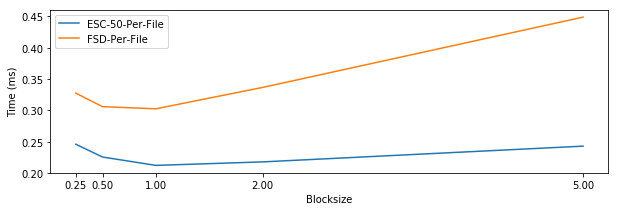
\includegraphics[width=0.45\textwidth]{figures/dataset-load-time.png}
    \caption{Caption}
    \label{fig:load-time}
\end{figure}

The datasets chosen for training are ideally clean, uniform and have about an equal number of each class instance. 

The system depends on the ability of the machine learning agent to be able to
match between acoustic features and the text queries. Its performance depends on
both the size of the database and the specificity of the query. To examine
performance across environments, we choose a clean and a dirty database: ESC-50
\cite{Piczak2015} and Freesound.

\subsubsection{ESC-50}
This clean database is made available on GitHub for environmental sound
classification. It is maintained such that the tag vocabulary is fixed and each
audio document attempts to only contains a single object in it. Each document is
5 seconds long and audio quality in terms of samplerate and recording noise is
normalized across the database. This makes for a very clean database with little
noise in both audio and annotation. It has 50 semantic classes with 40 examples
per class arranged into 5 major categories. However, the major categories do not
match the Gaver taxonomy and so were manually separated as in Table
~\ref{tab:relabel}. The database's sound documents come from the Freesound
project with the author providing uniform tags and normalizing the audio
manually \cite{Font2013}.

\subsubsection{Freesound}
The Freesound database is made up entirely of user-submitted and tagged audio documents. This is used to test the efficacy of the method on a real-world unstructured database. The documents in the database are in a variety of audio formats and lengths. Additionally, a portion of the documents contain multiple audio objects that overlap.

\subsection{Results}

\subsubsection{Preprocessing}


\subsubsection{Encoding Results}
\begin{figure}[h]
    \centering
    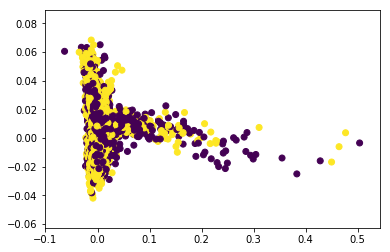
\includegraphics[width=0.45\textwidth]{figures/pca-cluster-hl.png}
    \caption{2D clustering of features using PCA.}
    \label{fig:pcahl}
\end{figure}

\begin{table}[t]
    \centering
    \begin{tabular}{c|cc}
    \textbf{Window} & \textbf{Read} & \textbf{Process} \\ \hline
    250              & 7840           & 37318                    \\
    2000             & 2413           & 4831                   
    \end{tabular}
    \caption{The average read and processing time in ms for 400 documents.}
    \label{tab:base-time}
\end{table}

\subsubsection{Training Evaluation}

\begin{figure}
    \centering
    \includegraphics[width=0.45\textwidth]{example-image-a}
    \caption{Comparative training time between PAMIR, WARP, and ECHO (what we're calling this system?)}
    \label{fig:my-label}
\end{figure}

\begin{figure}
    \centering
    \includegraphics[width=0.45\textwidth]{example-image-a}
    \caption{Plot of training iterations needed before getting diminishing returns (comparative between classifiers)}
    \label{fig:learning-curve}
\end{figure}

\subsubsection{Representation Experiments}

\begin{table}[]
    \begin{tabular}{llllll}
    Classifier/Window       & 250 ms & 500 ms & 1 s   & 2 s  & 5 s   \\
    Deep Neural Nets        & 0.628  & 0.653  & 0.656 &      &       \\
    Random Forest           & 0.66   & 0.68   & 0.68  & 0.64 & 0.69  \\
    K-Nearest Neighbors     & 0.61   & 0.62   & 0.62  & 0.65 & 0.64 \\
    Support Vector Machine  & 0.62   & 0.64   & 0.62  & 0.62 & 0.67   
    \end{tabular}
\end{table}

Classifier performance at different window sizes and features (remember, have run wavenet)

\begin{figure}[h]
    \centering
    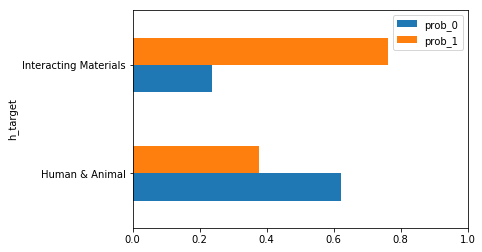
\includegraphics[width=0.45\textwidth]{figures/knn-prob-plot.png}
    \caption{Plot of average probabilities for each class of the misclassified documents at the top level.}
    \label{fig:a}
\end{figure}

\subsubsection{Pure Classification Performance}

Cross-validated performance of each subclassifier and performance of hierarchical

\subsubsection{Retrieval Performance (Time + Accuracy)}


\section{Conclusion}
The approach here shows promise, especially in the context of a retrieval
system. Using human perception as a model is an approach that had been pursued
in machine vision with success and it is only logical to do the same for machine
listening. By understanding the mechanisms by which we convert auditory signals
to brain signals, we can understand how the audio needs to be encoded for use in
machine hearing. One of the aspects of audio we have yet to optimally integrate
are temporal features which are of utmost importance in audio signals.

To this end, several representations were attempted in this work. The first was
just basic feature extraction from spectral representations of the audio using
librosa. Librosa allowed for many spectral and temporal features to be taken
from the signal though it is a slow process and may still not provide a good
feature set. To better emulate human perception, auto-encoders were attempted
next. The thought was that a neural network will be able to find latent
variables that are of better use than those extracted from usual means. However,
it was found that this approach did not bear out and hardly effected
performance.

Experiments were run comparing this approach to two off-the-shelf classifiers on
each layer of the hierarchy. The SVM classifier consistently under-performed and
will likely be removed from subsequent evaluations. A Random Forest Classifier
was consistently about equal to the neural networks it was evaluated against but
in nearly every case, the network was able to beat its precision score.

Overall, this study provided insights into the complexity of autonomous audio
analysis and the challenges that are still facing the field. of these
challenges, it seems that representation is the most pressing. It appears though
that the current direction of studying human perception mechanisms and emulating
them will prove optimal.

